% !TeX root = RJwrapper.tex
\title{Partitioned Local Depth (PaLD) Clustering Analyses in R}
\author{by Lucy D'Agostino McGowan, Katherine Moore, and Kenneth Berenhaut}

\maketitle

\abstract{%
An abstract of less than 150 words.
}

\hypertarget{introduction}{%
\subsection{Introduction}\label{introduction}}

\begin{itemize}
\tightlist
\item
  Describe PaLD (Ken \& Kate?) \citep{berenhaut2022social}
\end{itemize}

We present a new package, \CRANpkg{pald}, for calculating partitioned
local depth (PaLD) probabilities, implementing clustering analyses, and
creating data visualizations to represent the clusters. This paper will
describe how to use the package as well as walk through two examples.

\hypertarget{pald}{%
\subsection{pald}\label{pald}}

The main functions in \CRANpkg{pald} package can be split into 3
categories:

\begin{enumerate}
\def\labelenumi{\arabic{enumi}.}
\tightlist
\item
  Helper functions to organize data into the correct format, into
  distance matrices and then cohesion matrices
\item
  Functions that convert a cohesion matrix into a variety of useful
  formats, including partitioned local depths, clusters, and graphs
\item
  Plotting functions
\end{enumerate}

In addition, the package provides a number of pertinent example data
sets commonly used to demonstrate cluster algorithms, including a
synthetic data set of two-dimensional points created by
\citet{gionis1clustering} to demonstrate clustering aggregation, a
sample of walking distances from a pump in the infamous cholera outbreak
\citep{cholera}, clustering data generated from the scikit-learn Python
package \citep{pedregosa2011scikit}, and data compiled by \cite{tissue}
of tissue gene expressions.

While it is not a necessity, the \CRANpkg{pald} package is designed to
function well with the pipe operator, \texttt{\textbar{}\textgreater{}}.
This functionality will be demonstrated below.

\hypertarget{helper-functions-to-create-contribution-matrix}{%
\subsubsection{Helper functions to create contribution
matrix}\label{helper-functions-to-create-contribution-matrix}}

For demonstration purposes, below is a sample data frame with two
variables, \texttt{x1} and \texttt{x2}. The methods put forth here work
on data frames with higher dimensions, as described in the
\textbf{Examples} section; we are simply choosing a small data frame
here for demonstration purposes.

\begin{Schunk}
\begin{Sinput}
library(pald)
df <- data.frame(
  x1 = c(6, 8, 11, 16, 4),
  x2 = c(5, 4, 13, 7, 18)
)
rownames(df) <- c("A", "B", "C", "D", "E")
\end{Sinput}
\end{Schunk}

The first step needed to calculate the partitioned local depths is to
construct a \emph{distance matrix}. If the data are already in this
form, the user can skip to the next step. The \texttt{dist()} function
converts an input data frame into a distance matrix, as demonstrated
below.

\begin{Schunk}
\begin{Sinput}
d <- dist(df)
\end{Sinput}
\end{Schunk}

This will create an \(n\times n\) distance matrix, where \(n\)
corresponds to the number of observations in the original data frame, in
this example \(n = 5\). This distance matrix can then be passed to the
\texttt{cohesion\_matrix()} function in order to calculate the pairwise
cohesion values. Cohesion is an interpretable probability that reflects
the strength of alignment of two points. Again, if the user begins with
a distance matrix, they can skip the first step and simply input the
distance matrix into this function.

\begin{Schunk}
\begin{Sinput}
d <- dist(df)
cohesion_matrix(d)
\end{Sinput}
\begin{Soutput}
#>        A      B         C         D         E
#> A 0.2875 0.1625 0.0000000 0.0500000 0.0000000
#> B 0.1625 0.2875 0.0000000 0.0500000 0.0000000
#> C 0.0000 0.0000 0.3083333 0.1833333 0.1000000
#> D 0.0500 0.0500 0.1750000 0.3000000 0.0000000
#> E 0.0000 0.0000 0.1000000 0.0000000 0.2333333
\end{Soutput}
\end{Schunk}

Equivalently, the user can use the native pipe
\texttt{\textbar{}\textgreater{}} as follows.

\begin{Schunk}
\begin{Sinput}
df |>
  dist() |>
  cohesion_matrix()
\end{Sinput}
\begin{Soutput}
#>        A      B         C         D         E
#> A 0.2875 0.1625 0.0000000 0.0500000 0.0000000
#> B 0.1625 0.2875 0.0000000 0.0500000 0.0000000
#> C 0.0000 0.0000 0.3083333 0.1833333 0.1000000
#> D 0.0500 0.0500 0.1750000 0.3000000 0.0000000
#> E 0.0000 0.0000 0.1000000 0.0000000 0.2333333
\end{Soutput}
\end{Schunk}

The \emph{cohesion matrix} output by the \texttt{cohesion\_matrix()} is
the main input for the majority of the remaining functions.

\hypertarget{functions-that-convert-a-cohesion-matrix-into-useful-formats}{%
\subsubsection{Functions that convert a cohesion matrix into useful
formats}\label{functions-that-convert-a-cohesion-matrix-into-useful-formats}}

From the \emph{cohesion matrix}, a variety of useful quantities can be
calculated. Below, we create a cohesion matrix using the functions
described in the previous section.

\begin{Schunk}
\begin{Sinput}
d |>
  dist() |>
  cohesion_matrix() -> cohesion
\end{Sinput}
\end{Schunk}

To calculate the \emph{clusters} that each point will fall into, we can
use the \texttt{community\_clusters()} function. This will output a data
frame with two columns, the first will correspond to the \texttt{point},
as identified by the row name of the original input data frame,
\texttt{df}, the second will identify the \texttt{cluster} that each
point belongs to.

\begin{Schunk}
\begin{Sinput}
community_clusters(cohesion)
\end{Sinput}
\begin{Soutput}
#>   point cluster
#> A     A       1
#> B     B       1
#> C     C       2
#> D     D       2
#> E     E       3
\end{Soutput}
\end{Schunk}

In this example, three clusters are identified with these five points.
Points \texttt{A} and \texttt{B} fall into cluster 1. Points \texttt{C}
and \texttt{D} into cluster 2, and point \texttt{E} in cluster 3.

The \texttt{local\_depths()} function calculates the \emph{depths} of
each point, outputting a vector of local depths. Local depth is an
interpretable probability which reflects aspects of relative position
and centrality via distance comparisons (i.e., \(d(z, x) < d(z, y)\)).

\begin{Schunk}
\begin{Sinput}
local_depths(cohesion)
\end{Sinput}
\begin{Soutput}
#>         A         B         C         D         E 
#> 0.4062500 0.5416667 0.3833333 0.4687500 0.7000000
\end{Soutput}
\end{Schunk}

In this case, the deepest point is \texttt{C}.

The \texttt{strong\_threshold()} function will calculate the cohesion
threshold for strong ties. This is equal to half the average of the
diagonal cohesion matrix. This is a threshold that may be used to
distinguish between strong and weak ties.

\begin{Schunk}
\begin{Sinput}
strong_threshold(cohesion)
\end{Sinput}
\begin{Soutput}
#> [1] 0.14
\end{Soutput}
\end{Schunk}

In this case, the threshold is \texttt{0.14}.

The \texttt{any\_isolated()} function will check whether there are any
isolated points that will inadvertently be dropped by a graph.

\begin{Schunk}
\begin{Sinput}
any_isolated(cohesion)
\end{Sinput}
\end{Schunk}

Here, there are no isolated points.

The function \texttt{cohesion\_strong()} will update the cohesion matrix
to set all weak ties to zero (via the \texttt{strong\_threshold()}
function). Optionally, the matrix will also be symmetrized, with the
default parameter \texttt{symmetric\ =\ TRUE}.

\begin{Schunk}
\begin{Sinput}
cohesion_strong(cohesion)
\end{Sinput}
\begin{Soutput}
#>        A      B     C     D      E
#> A 0.3000 0.1625 0.000 0.000 0.0000
#> B 0.1625 0.2875 0.000 0.000 0.0000
#> C 0.0000 0.0000 0.300 0.175 0.0000
#> D 0.0000 0.0000 0.175 0.300 0.0000
#> E 0.0000 0.0000 0.000 0.000 0.2125
\end{Soutput}
\end{Schunk}

Finally, the \texttt{community\_graphs()} function takes the cohesion
matrix and creates \CRANpkg{igraph} objects, graphs that describes the
relationship between the points. This function will output a list of
three objects:

\begin{itemize}
\tightlist
\item
  \texttt{G}: the weighted (community) graph whose edge weights are
  mutual cohesion
\item
  \texttt{G\_strong}: the weighted (community) graph consisting of edges
  for which mutual cohesion is greater than the threshold for strong
  ties
\item
  \texttt{layout}: the graph layout, using the Fruchterman Reingold (FR)
  force-directed graph drawing for the graph \texttt{G}
\end{itemize}

\begin{Schunk}
\begin{Sinput}
graphs <- community_graphs(cohesion)
graphs[["G_strong"]]
\end{Sinput}
\begin{Soutput}
#> IGRAPH 261f39e UNW- 5 2 -- 
#> + attr: name (v/c), weight (e/n)
#> + edges from 261f39e (vertex names):
#> [1] A--B C--D
\end{Soutput}
\end{Schunk}

Here we see that there are two connected components, points \texttt{A}
and \texttt{B}, which form the first cluster, and points \texttt{D} and
\texttt{C} which form the second.

\hypertarget{plotting-functions}{%
\subsection{Plotting functions}\label{plotting-functions}}

The final category of function is functions for data visualization. We
can begin by visualizing the points in data frame \texttt{df} (Figure
\ref{fig:fig1}).

\begin{Schunk}
\begin{Sinput}
library(ggplot2)
ggplot(df, aes(x1, x2)) +
  geom_text(label = rownames(df))
\end{Sinput}
\begin{figure}
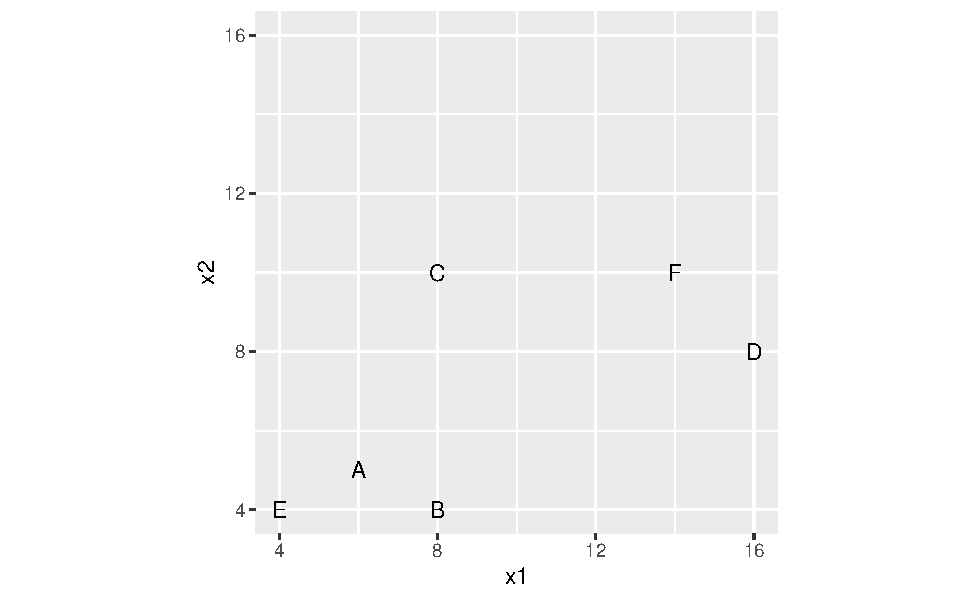
\includegraphics{manuscript_files/figure-latex/fig1-1} \caption[Visualize the points from data frame `df`]{Visualize the points from data frame `df`}\label{fig:fig1}
\end{figure}
\end{Schunk}

We can then pass the cohesion matrix to the
\texttt{plot\_community\_graphs()} function to view the relationship
between points (Figure \ref{fig:fig2}).

\begin{Schunk}
\begin{Sinput}
df |>
  dist() |>
  cohesion_matrix() |>
  plot_community_graphs()
\end{Sinput}
\begin{figure}
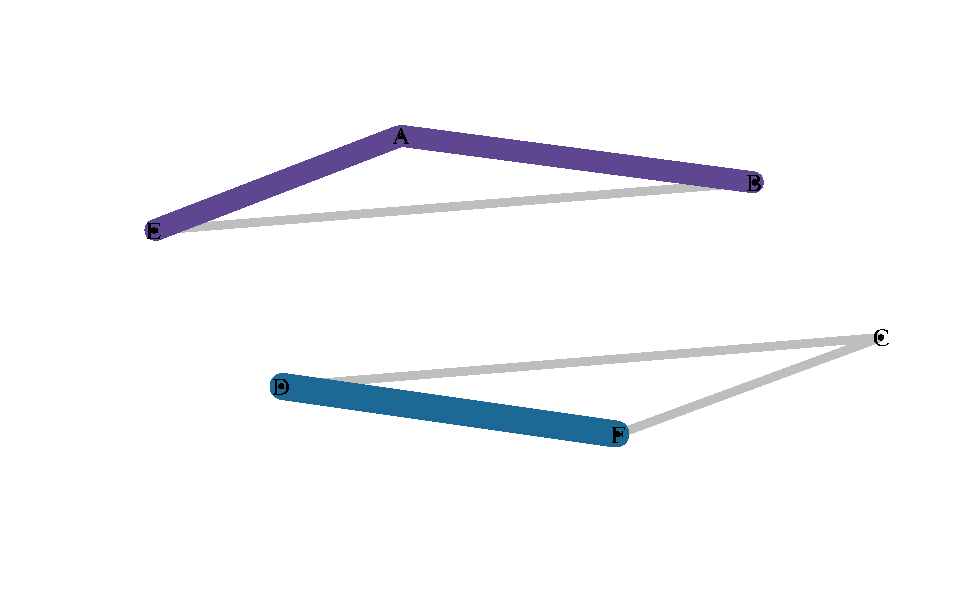
\includegraphics{manuscript_files/figure-latex/fig2-1} \caption[PaLD graph displaying the relationship between the points in data frame `df`]{PaLD graph displaying the relationship between the points in data frame `df`}\label{fig:fig2}
\end{figure}
\end{Schunk}

The \texttt{layout} argument allows the user to pass a matrix to dictate
the layout of the graph. For example, if we wanted the graph to match
the visualization displayed in Figure \ref{fig:fig1}, we can pass
\texttt{as.matrix(df)}, or a matrix of the data frame \texttt{df} to the
\texttt{layout} argument (Figure \ref{fig:fig3}.

\begin{Schunk}
\begin{Sinput}
df |>
  dist() |>
  cohesion_matrix() |>
  plot_community_graphs(layout = as.matrix(df))
\end{Sinput}
\begin{figure}
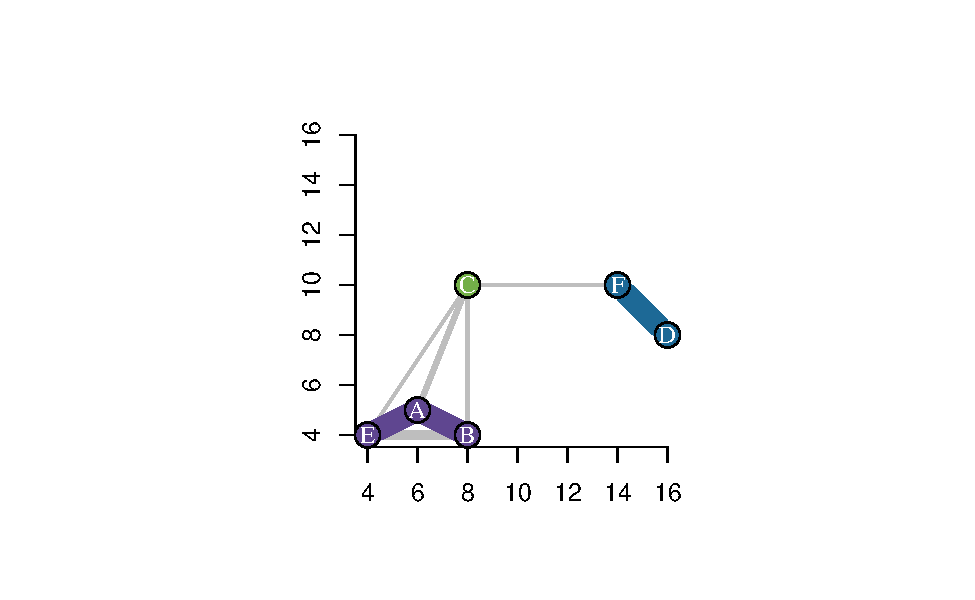
\includegraphics{manuscript_files/figure-latex/fig3-1} \caption[PaLD graph displaying the relationship between the points in data frame `d`, matching the original layout in Figure 1]{PaLD graph displaying the relationship between the points in data frame `d`, matching the original layout in Figure 1}\label{fig:fig3}
\end{figure}
\end{Schunk}

This \texttt{plot\_community\_graphs()} function will also permit
parameters that can be passed to the \texttt{plot.igraph()} function.
For example, to add axes to the graph, the user can pass the
\texttt{axes\ =\ TRUE} argument to the \texttt{...} in the
\texttt{plot\_community\_graphs()} function (Figure \ref{fig:fig4}).

\begin{Schunk}
\begin{Sinput}
df |>
  dist() |>
  cohesion_matrix() |>
  plot_community_graphs(layout = as.matrix(df),
                        axes = TRUE)
\end{Sinput}
\begin{figure}
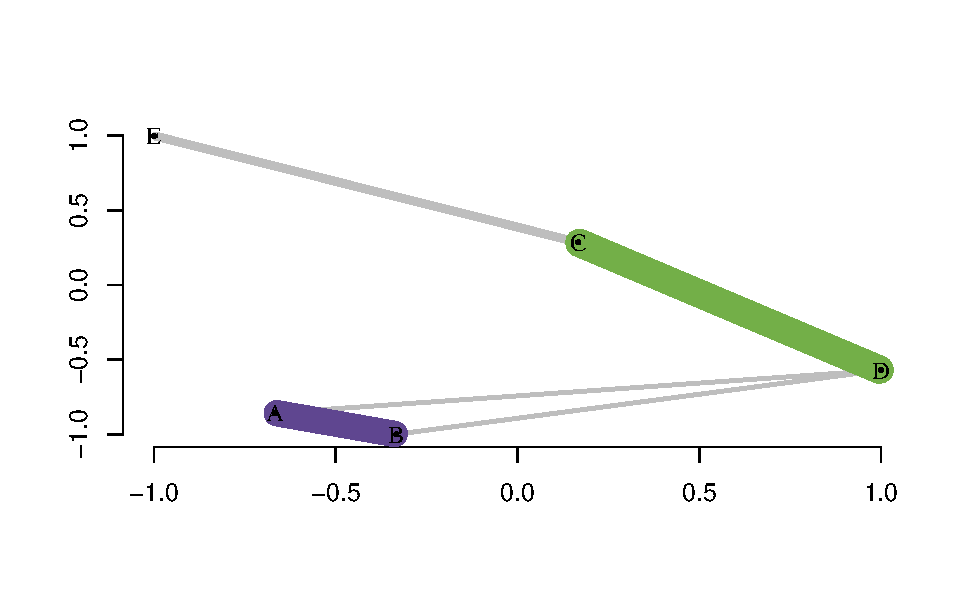
\includegraphics{manuscript_files/figure-latex/fig4-1} \caption[PaLD graph displaying the relationship between the points in data frame `d`, matching the original layout in Figure 1, adding axes]{PaLD graph displaying the relationship between the points in data frame `d`, matching the original layout in Figure 1, adding axes}\label{fig:fig4}
\end{figure}
\end{Schunk}

\hypertarget{examples}{%
\subsection{Examples}\label{examples}}

We will demonstrate the utility of the \CRANpkg{pald} package in two
clustering examples.

\hypertarget{clustering-tissue-gene-expression-data}{%
\subsubsection{Clustering tissue gene expression
data}\label{clustering-tissue-gene-expression-data}}

The first example if from a subset of tissue gene expression data from
\citet{zilliox2007gene}, \citet{mccall2011gene}, and
\citet{mccall2014gene}, obtained from the \textbf{tissuesGeneExpression}
bioconductor package \citep{tissue}. A cohesion matrix was created using
this data set and is included the \CRANpkg{pald} package in an object
called \texttt{tissue\_cohesion\_matrix}.

The \texttt{tissue\_cohesion\_matrix} object is a cohesion matrix with
189 rows and 189 columns.

We can use this contribution matrix to display the relationship between
tissue samples using the \texttt{plot\_community\_graphs()} function
(Figure \ref{fig:fig5}). For clarity of the display, we show how to only
include a random set of the vertex labels. We can pass this random set
through the \texttt{...} to the \texttt{plot.igraph}
\texttt{vertex.label} parameter.

\begin{Schunk}
\begin{Sinput}
set.seed(1)

labels <- rownames(tissue_cohesion_matrix)
labels[sample(1:189, 125)] <- ""
plot_community_graphs(tissue_cohesion_matrix,
                      vertex.label = labels,
                      vertex.size = 4)
\end{Sinput}
\begin{figure}
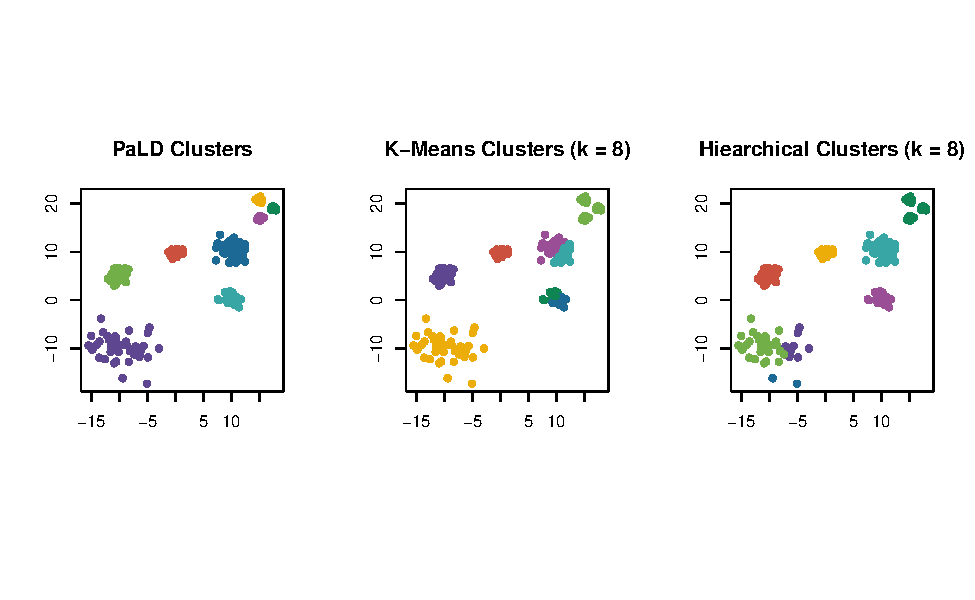
\includegraphics{manuscript_files/figure-latex/fig5-1} \caption[PaLD clustering of tissue data]{PaLD clustering of tissue data}\label{fig:fig5}
\end{figure}
\end{Schunk}

The \texttt{community\_clusters()} function can be used to identify the
clusters of each tissue sample. Since the output is a data frame, we can
summarize the clusters using commonly used data analysis techniques. For
demonstration purposes, we will use the \CRANpkg{dplyr} package to
summarize the contribution of clusters.

\begin{Schunk}
\begin{Sinput}
library(dplyr)
community_clusters(tissue_cohesion_matrix) %>%
  group_by(cluster, point) %>%
  count()
\end{Sinput}
\begin{Soutput}
#> # A tibble: 19 x 3
#> # Groups:   cluster, point [19]
#>    cluster point           n
#>      <dbl> <chr>       <int>
#>  1       1 endometrium    15
#>  2       1 kidney         39
#>  3       2 hippocampus    31
#>  4       3 cerebellum     26
#>  5       4 cerebellum      1
#>  6       5 colon          33
#>  7       6 colon           1
#>  8       7 liver           7
#>  9       8 cerebellum      1
#> 10       9 liver          17
#> 11      10 cerebellum      2
#> 12      11 liver           2
#> 13      12 cerebellum      1
#> 14      13 cerebellum      4
#> 15      14 cerebellum      2
#> 16      15 cerebellum      1
#> 17      16 placenta        2
#> 18      17 placenta        1
#> 19      18 placenta        3
\end{Soutput}
\end{Schunk}

From this, we can glean that cluster one consists of two types of
tissue, the kidney and endometrium. Cluster two is comprised of only the
hippocampus.

\hypertarget{clustering-generated-data}{%
\subsubsection{Clustering generated
data}\label{clustering-generated-data}}

The \CRANpkg{pald} includes three randomly generated data frames
corresponding to plots from \citet{berenhaut2022social}:

\begin{itemize}
\tightlist
\item
  \texttt{exdata1} is a data set consisting of 8 points to recreate
  Figure 1 in \citet{berenhaut2022social}
\item
  \texttt{exdata2} is a data set consisting of 16 points to recreate
  Figure 2 in \citet{berenhaut2022social}
\item
  \texttt{exdata3} is a data set consisting of 240 points to recreate
  Figure 4D in \citet{berenhaut2022social}
\end{itemize}

Here, we will demonstrate how to use \texttt{exdata3}. These points were
generated from bivariate normal distributions with varying means and
variances.

\begin{Schunk}
\begin{Sinput}
exdata_cohesion_matrix <- exdata3 |>
  dist() |>
  cohesion_matrix()
\end{Sinput}
\end{Schunk}

When plotting the \texttt{exdata3} PaLD graph, we want the layout to
match the layout of the original data, so we will pass
\texttt{as.matrix(exdata3)} to the \texttt{layout} parameter in the
\texttt{plot\_community\_graphs()} function. Additionally, here the row
names are meaningless, they just correspond to the location of the
generated data, so we can remove the labels on the plot by setting
\texttt{show\_labels\ =\ FALSE}. The \texttt{only\_strong} parameter
will only display the strongly connected edges. Additionally, we can
optionally pass parameters through the \texttt{...} to
\texttt{plot::igraph} function; for example, to increase the vertex size
we can set \texttt{vertex.size\ =\ 5}. Figure \ref{fig:fig6} shows this.

\begin{Schunk}
\begin{Sinput}
plot_community_graphs(exdata_cohesion_matrix,
                layout = as.matrix(exdata3),
                show_labels = FALSE, 
                only_strong = TRUE,
                vertex.size = 5)
\end{Sinput}
\begin{figure}
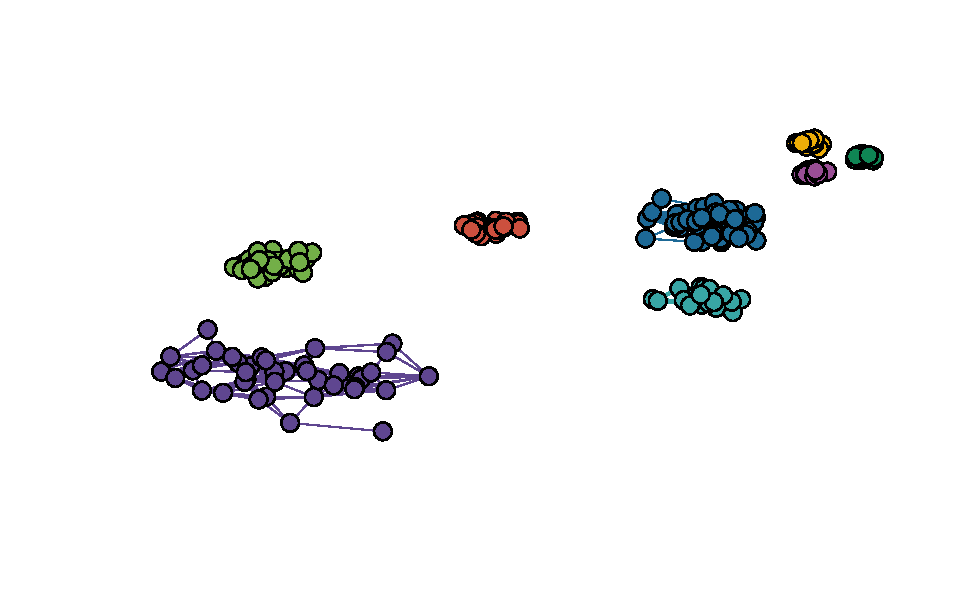
\includegraphics{manuscript_files/figure-latex/fig6-1} \caption[PaLD clustering of randomly generated example data (from Figure 4D from Berenhaut et al]{PaLD clustering of randomly generated example data (from Figure 4D from Berenhaut et al. (2022))}\label{fig:fig6}
\end{figure}
\end{Schunk}

The ability of the PaLD algorithm to discern clusters is demonstrated
here.

\hypertarget{summary}{%
\subsection{Summary}\label{summary}}

This paper introduces the \CRANpkg{pald} package, demonstrating it's
utility for providing a parameter-free clustering algorithm that can
easily be applied to any data set.

\bibliography{RJreferences}


\address{%
Lucy D'Agostino McGowan\\
Wake Forest University\\%
Winston-Salem, NC\\ 27106\\
%
%
%
\href{mailto:mcgowald@wfu.edu}{\nolinkurl{mcgowald@wfu.edu}}%
}

\address{%
Katherine Moore\\
Wake Forest Unversity\\%
Winston-Salem, NC\\ 27106\\
%
%
%
\href{mailto:mooreke@wfu.edu}{\nolinkurl{mooreke@wfu.edu}}%
}

\address{%
Kenneth Berenhaut\\
Wake Forest University\\%
Winston-Salem, NC\\ 27106\\
%
%
%
\href{mailto:berenhks@wfu.edu}{\nolinkurl{berenhks@wfu.edu}}%
}
